\pdfoutput=1
\pdfcompresslevel=9
\documentclass[a4paper,onecolumn,oneside,11pt,wide,floatssmall]{mwrep}
\usepackage{algorithm}
\usepackage{algpseudocode}
\usepackage{amsmath}
\usepackage{amsfonts}
\usepackage{amssymb}
\usepackage{amsthm}
\usepackage{float}
\usepackage{geometry}
\usepackage{listings}
\usepackage[pdftex]{color,graphicx}
\usepackage{polski}
\usepackage[pdftex, bookmarks=false]{hyperref}
\usepackage[table]{xcolor}
\usepackage[T1]{fontenc}
\usepackage[utf8x]{inputenc}
\usepackage[sort, compress]{cite}

\def\url#1{{ \tt #1}}
\def\C{{\rm C}\,}
\def\E{{\rm E}\,}
\def\sgn{{\rm sgn}\,}

% marginesy
\textwidth\paperwidth
\advance\textwidth -55mm
\oddsidemargin-0.9in
\advance\oddsidemargin 33mm
\evensidemargin-0.9in
\advance\evensidemargin 33mm
\topmargin -1in
\advance\topmargin 25mm
\setlength\textheight{48\baselineskip}
\addtolength\textheight{\topskip}
\marginparwidth15mm

\clubpenalty=10000 % to kara za sierotki
\widowpenalty=10000 % nie pozostawia wdów
\brokenpenalty=10000 % nie dzieli wyrazów pomiędzy stronami
\sloppy

\tolerance4500
\pretolerance250
\hfuzz=1.5pt
\hbadness1450

% ŻYWA PAGINA
\renewcommand{\chaptermark}[1]{\markboth{\scshape\small\bfseries \
#1}{\small\bfseries \ #1}}
\renewcommand{\sectionmark}[1]{\markboth{\scshape\small\bfseries\thesection.\
#1}{\small\bfseries\thesection.\ #1}}
\newcommand{\headrulewidth}{0.5pt}
\newcommand{\footrulewidth}{0.pt}
\pagestyle{uheadings}

\theoremstyle{definition}
\newtheorem{defn}{Definicja}[section]
\newtheorem{conj}{Teza}[section]
\newtheorem{conjmain}{Teza}
\newtheorem{exmp}{Przykład}[section]

\theoremstyle{plain}% default
\newtheorem{thm}{Twierdzenie}[section]
\newtheorem{lem}[thm]{Lemat}
\newtheorem{prop}[thm]{Hipoteza}
\newtheorem*{cor}{Wniosek}

\theoremstyle{remark}
\newtheorem*{rem}{Uwaga}
\newtheorem*{note}{Uwaga}
\newtheorem{case}{Przypadek}

\definecolor{ListingBackground}{rgb}{0.95,0.95,0.95}

\begin{document}

\renewcommand*\lstlistingname{Wydruk}
\renewcommand*\lstlistlistingname{Spis wydruków}

\pagenumbering{roman}
\renewcommand{\baselinestretch}{1.0}
\raggedbottom
\begin{titlepage}
    % Strona tytułowa
    \vbox to\textheight{\hyphenpenalty=10000
    \begin{center}
	\begin{tabular}{p{107mm} p{9cm}}
	    \begin{minipage}{9cm}
	      \begin{center}
	      Politechnika Warszawska \\
	      Wydział Elektroniki i~Technik Informacyjnych \\
	      Instytut Informatyki
	      \end{center}
	    \end{minipage}
	    &
	    \begin{minipage}{8cm}
	    \begin{flushleft}
	     \footnotesize
	      Rok akademicki 2013/2014
	    \vspace*{2.75\baselineskip}
	    \end{flushleft}
	    \end{minipage} \\
	\end{tabular}
	\vspace*{3.75\baselineskip}
	\par\vspace{\smallskipamount}
	\vspace*{2\baselineskip}{\LARGE Praca dyplomowa magisterska\par}
	\vspace{3\baselineskip}{\LARGE\strut Adam Stelmaszczyk\par}
	\vspace*{2\baselineskip}{\huge\bfseries DE/mid -- nowy wariant algorytmu ewolucji różnicowej wykorzystujący punkt środkowy populacji\par}

	\vspace*{2\baselineskip}
	\hfill\mbox{}\par\vspace*{\baselineskip}\noindent
	\begin{tabular}[b]{@{}p{3cm}@{\ }l@{}}
	    {\large\hfill } & {\large }
	\end{tabular}
	\hfill
	\begin{tabular}[b]{@{}l@{}}
	Opiekun pracy: \\[\smallskipamount]
	{\large prof. nzw. dr hab. Jarosław Arabas}
	\end{tabular}\par
	\vspace*{2\baselineskip}
    \begin{tabular}{p{\textwidth}}
    \begin{flushleft}
	\begin{minipage}{7cm}
	Ocena \dotfill
	\par\vspace{1.6\baselineskip}
	\dotfill
	\par\noindent
	\centerline{\footnotesize Podpis Przewodniczącego} \par
	\centerline{\footnotesize Komisji Egzaminu Dyplomowego}\par
	\end{minipage}
    \end{flushleft}
    \end{tabular}
    \end{center}}

    % Życiorys
    \newpage\thispagestyle{empty}
    \begin{tabular}{p{5cm} p{12cm}}
    \begin{minipage}{5cm}
    \center
    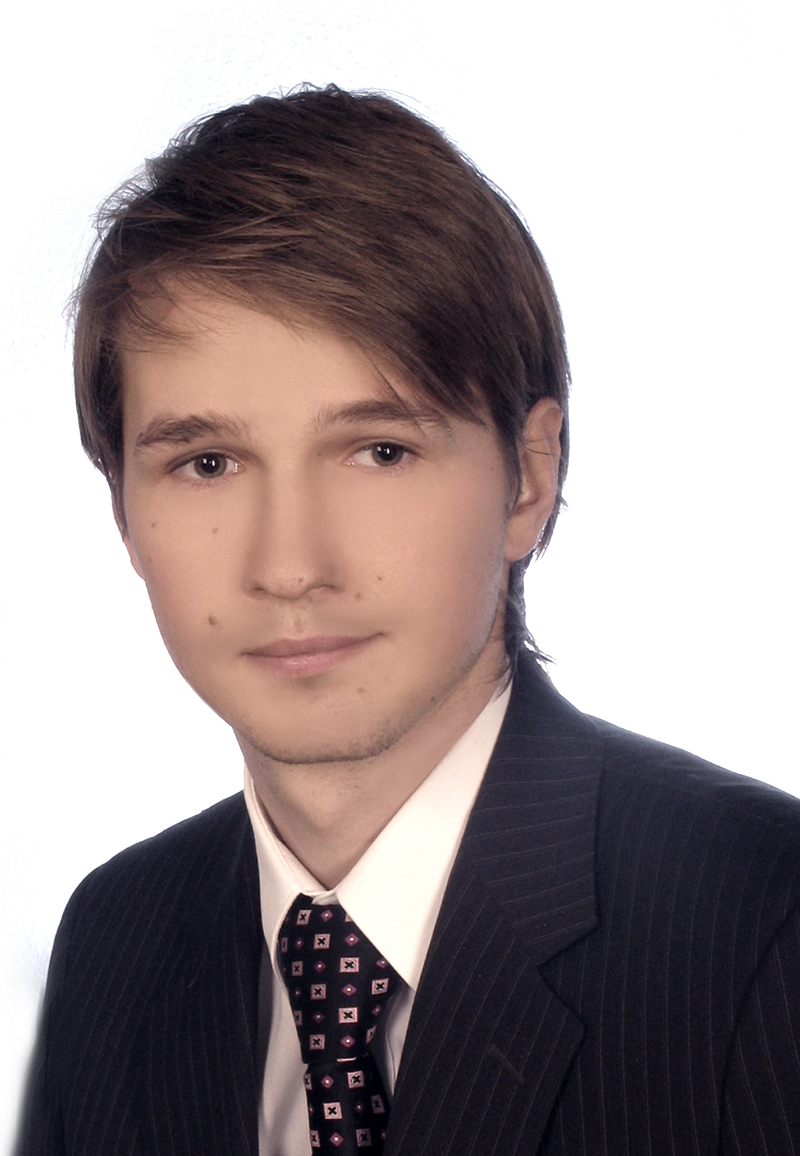
\includegraphics[height=6.5cm,width=4.5cm]{img/foto.jpg}
    \end{minipage}
    &
    \begin{minipage}{12cm}
    \begin{flushleft}
    \par\noindent\vspace{1\baselineskip}
    \begin{tabular}[h]{l l}
    {\normalsize\it Specjalność:} & \normalsize Inżynieria Systemów Informacyjnych 
    \end{tabular}
    \par\noindent\vspace{1\baselineskip}
    \begin{tabular}[h]{l l}
    {\normalsize\it Data urodzenia:} & {\normalsize 12 stycznia 1990~r.}
    \end{tabular}
    \par\noindent\vspace{1\baselineskip}
    \begin{tabular}[h]{l l}
    {\normalsize\it Data rozpoczęcia studiów:} & {\normalsize 1 października 2009 r.}
    \end{tabular}
    \par\noindent\vspace{1\baselineskip}
    \end{flushleft}
    \end{minipage}
    \end{tabular}
    \vspace*{1\baselineskip}
    \begin{center}
	{\large\bfseries Życiorys}\par\bigskip
    \end{center}

    \indent
Urodziłem się 12 stycznia 1990 roku w Piotrkowie Trybunalskim. Ukończyłem Szkołę Podstawową
nr 33, Gimnazjum nr 11 oraz Liceum Ogólnokształcące im. Jana Kochanowskiego w Warszawie, gdzie
uczęszczałem do klasy o profilu matematyczno--fizyczno--informatycznym.
W październiku 2009 roku rozpocząłem studia na Wydziale Elektroniki i Technik Informacyjnych
Politechniki Warszawskiej na kierunku Informatyka. W lutym 2013 roku uzyskałem tytuł inżyniera.

    \par
    \vspace{3\baselineskip}
    \hfill\parbox{15em}{{\small\dotfill}\\[-.3ex]
    \centerline{\footnotesize podpis studenta}}\par
    \vspace{2\baselineskip}
    \begin{center}
 	{\large\bfseries Egzamin dyplomowy} \par\bigskip
    \end{center}
    \par\noindent\vspace{1\baselineskip}
    Złożył egzamin dyplomowy w dn. \dotfill
    \par\noindent\vspace{1\baselineskip}
    Z wynikiem \dotfill
    \par\noindent\vspace{1\baselineskip}
    Ogólny wynik studiów \dotfill
    \par\noindent\vspace{1\baselineskip}
    Dodatkowe wnioski i uwagi Komisji \dotfill
  
    % Streszczenie
    \newpage\thispagestyle{empty}
    \vspace*{2\baselineskip}
    \begin{center}
	{\large\bfseries Streszczenie}\par\bigskip
    \end{center}

    {\itshape
W pracy przeanalizowano działanie znanych wariantów algorytmu ewolucji różnicowej~--~DE/rand
oraz DE/best. W celu poprawienia wyników zaproponowano nowy wariant nazwany DE/mid. 
Żeby porównanie jakości algorytmów było sprawiedliwe, każdemu z wariantów ustalono taki sam zasięg
mutacji poprzez dobranie odpowiedniego współczynnika skalującego.
Na podstawie przeprowadzonych testów stwierdzono poprawę jakości uzyskiwanych wyników na 6 z 7 
wielowymiarowych funkcji testowych z zestawu BBOB 2013.}
    \vspace*{1\baselineskip}

    \noindent{\bf Słowa kluczowe}: {\itshape ewolucja różnicowa, algorytm ewolucyjny, genetyczny, optymalizacja globalna}
    \par
    \vspace{4\baselineskip}
    \begin{center}
	{\large\bfseries Abstract}\par\bigskip
    \end{center}
    \noindent{\bf Title}: {\itshape DE/mid -- new variant of differential evolution algorithm using the midpoint of the population}\par
    \vspace*{1\baselineskip}
    {\itshape
This thesis analyzes behaviour of known differential evolution variants -- DE/rand and DE/best.
In order to achieve better performance, new variant named DE/mid has been introduced.
To ensure a fair comparison between algorithms, mutation of every algorithm variant had exactly
the same range. 
Tests indicated improvement of results quality on 6 out of 7 high-dimensional
testing functions from BBOB 2013 testbed.}
    \vspace*{1\baselineskip}

    \noindent{\bf Key words}: {\itshape differential evolution, evolutionary, genetic algorithm, global optimization
}

\end{titlepage}

\tableofcontents

\newpage
\pagenumbering{arabic}
\setcounter{page}{1}

\chapter{Wstęp}

\section{Słownik pojęć i oznaczeń}

\chapter{Ewolucja różnicowa}

Klasyczna ewolucja różnicowa DE/rand oraz jej odmiana DE/mid różnią się jedynie operatorem mutacji.
W poniższych rozdziałach przedstawiono operatory mutacji dla DE/rand/k, DE/mid/k, DE/rand/$\infty$, DE/mid/$\infty$
oraz wyprowadzono wzory na współczynniki skalujące.

\section{DE/rand}

W DE/rand/1, mutant $i$-tego osobnika w populacji $P$~o~$n$~osobnikach powstaje w następujący sposób \cite{decomposition}:
\begin{equation} \label{eq:derand1}
u_i = P_{i_1} + F(P_{i_2} - P_{i_3})
\end{equation}

$i_1, i_2, i_3$ to indeksy wylosowane zgodnie z rozkładem jednostajnym ze zbioru \\ 
$\{0, 1, \dots, n-1\}$. Zatem $P_{i_1}, P_{i_2}, P_{i_3}$ to rozwiązania wylosowane zgodnie z rozkładem jednostajnym z populacji $P$.
$F\in\mathbb{R_+}$ to współczynnik skalujący, w tej pracy ustalony na 0,9. \\

DE/rand/1 można uogólnić na DE/rand/k, w którym to dodajemy
$k \in \mathbb{N}$ wektorów różnicowych:
\begin{equation} \label{eq:derand}
u_i' = P_{i_1} + F_k\sum\limits_{j=1}^k (P_{i_{2j}} - P_{i_{2j+1}})
\end{equation}

Podobnie jak poprzednio, $i_1, i_2, \dots i_{2k+1}$ to indeksy wylosowane zgodnie z rozkładem jednostajnym ze zbioru 
$\{0, 1, \dots, n-1\}$. Zatem $P_{i_1}, P_{i_2}, \dots, P_{2k+1}$ to rozwiązania wylosowane zgodnie z rozkładem 
jednostajnym z populacji $P$. $F_k\in\mathbb{R_+}$ to współczynnik skalujący dla DE/rand/k. 
Żeby macierz kowariancji populacji w DE/rand/k nie zmieniała się wraz z zmianą $k$, 
macierz kowariancji mutanta $u_i'$ musi być taka sama jak macierz kowariancji mutanta $u_i$.
Można to osiągnąć tak dobierając $F_k$, aby było spełnione równanie:
\begin{equation} \label{eq:kowariancje}
\C[u_i] = \C[u_i']
\end{equation}

Osobniki są liniowo niezależne od siebie, dlatego:
\begin{align*}
\C[u_i] \overset{(\ref{eq:derand1})}{=} \C[P_{i_1} + F(P_{i_2} - P_{i_3})] = \C[P_{i_1}] + F^2(\C[P_{i_2}] + \C[P_{i_3}])
\end{align*}

$\forall{i}\hspace{1mm}\C[P_i] = \C[P]$, ponieważ każdy osobnik ma taki sam rozkład prawdopodobieństwa. Zatem:
\begin{equation} \label{eq:macierz_kow_mutanta}
\C[u_i] = \C[P] + F^2(\C[P] + \C[P]) = \C[P](2F^2 + 1)
\end{equation}

Rozwijając prawą stronę równania (\ref{eq:kowariancje}):
\begin{align*}
\C[u_i'] \overset{(\ref{eq:derand})}{=} \C[P_{i_1} + F_k\sum\limits_{j=1}^k (P_{i_{2j}} - P_{i_{2j+1}})] 
= \C[P_{i_1}] + F_k^2\C[\sum\limits_{j=1}^k (P_{i_{2j}} - P_{i_{2j+1}})] \\
= \C[P_{i_1}] + F_k^2\C[\sum\limits_{j=2}^{2k+1} P_{i_{j}}] \\
= \C[P](2kF_k^2 + 1)
\end{align*}

Podstawiając do (\ref{eq:kowariancje}):
\begin{align*}
\C[P](2F^2 + 1) = \C[P](2kF_k^2 + 1)
\end{align*}

Zakładając, że $\C[P] \neq \textbf{0}$:
\begin{align*}
F^2 = kF_k^2
\end{align*}

Obie strony są nieujemne, więc ostatecznie:
\begin{align*}
F_k = \frac{F}{\sqrt{k}}
\end{align*}

Zgodnie z centralnym twierdzeniem granicznym, $\frac{1}{{\sqrt{k}}}\sum\limits_{j=1}^k (P_{i_{2j}} - P_{i_{2j+1}})$ 
zbiega według rozkładu do $\mathcal{N}(0, \C[P])$ gdy $k \to \infty$. 
Dzięki temu, równanie mutanta DE/rand/$\infty$ można zapisać jako:
\begin{align*}
u_i = P_{i_1} + F_\infty \cdot v_\infty
\end{align*}

Gdzie $v_\infty \sim \mathcal{N}(0, \C[P])$. Wyznaczmy $F_\infty$.
\begin{align*}
\C[u_i] = \C[P_{i_1} + F_\infty \cdot v_\infty] \overset{(\ref{eq:macierz_kow_mutanta})}{=} \C[P](2F^2 + 1) \\
\C[P] + \C[F_\infty \cdot v_\infty] = \C[P](2F^2 + 1) \\
\C[F_\infty \cdot v_\infty] = 2F^2\C[P] \\
F_\infty^2 \C[P] = 2F^2\C[P] \\
F_\infty^2 = 2F^2 \\
F_\infty = \sqrt{2}F
\end{align*}

\section{DE/best}

\section{DE/mid}

W DE/mid/k mutant powstaje w następujący sposób:

\begin{equation} \label{eq:demid}
u_i'' = m + F_m\sum\limits_{j=1}^k (P_{i_{2j}} - P_{i_{2j+1}})
\end{equation}

Jedyną różnicą w porównaniu do DE/rand/k jest $m$, czyli punkt środkowy populacji:
\begin{equation} \label{eq:midpoint}
m = \frac{1}{n}\sum\limits_{j=1}^n P_j
\end{equation}

$F_m\in\mathbb{R_+}$ jest współczynnikiem skalującym dla DE/mid/k, analogicznym do $F$ dla DE/rand/1. 
Żeby macierz kowariancji populacji w DE/mid była taka sama jak w DE/rand/1, 
macierz kowariancji mutanta $u_i''$ musi być taka sama jak macierz kowariancji mutanta $u_i$.
Można to osiągnąć tak dobierając $F_m$, żeby było spełnione równanie:
\begin{equation} \label{eq:rownanie}
\C[u_i] = \C[u_i'']
\end{equation}

Rozwijając prawą stronę równania (\ref{eq:rownanie}):
\begin{align*}
\C[u_i''] \overset{(\ref{eq:demid})}{=} \C[m + F_m\sum\limits_{j=1}^k (P_{i_{2j}} - P_{i_{2j+1}})] \\
\overset{(\ref{eq:midpoint})}{=} \C[\frac{1}{n}\sum\limits_{j=1}^n P_j] + F_m^2\C[\sum\limits_{j=1}^k (P_{i_{2j}} - P_{i_{2j+1}})] 
= \frac{1}{n^2}n\C[P] + F_m^2\C[\sum\limits_{j=2}^{2k+1} P] = \C[P](2kF_m^2 + \frac{1}{n})
\end{align*}

Podstawiając do (\ref{eq:rownanie}):
\begin{align*}
\C[P](2F^2 + 1) = \C[P](2kF_m^2 + \frac{1}{n})
\end{align*}

Przy założeniu, że $\C[P] \neq \textbf{0}$:
\begin{align*}
2F^2 + 1 = 2kF_m^2 + \frac{1}{n} \\
F_m^2 = \frac{2F^2 + 1 - \frac{1}{n}}{2k}
\end{align*}

Obie strony są nieujemne, więc:
\begin{align} \label{eq:a}
F_m\ = \sqrt{\frac{2F^2 + 1 - \frac{1}{n}}{2k}}
\end{align}

Przyjmując $F=0,9$ z (\ref{eq:a}) wynika, że: \\
$F_m \approx 1,14$ dla $k=1$ i $n\to\infty$. \\

W DE/mid przesuwany jest punkt środkowy $m$ zamiast losowo wybranego osobnika $P_{i_1}$.
Punkt środkowy jest mniej zmienny, 
tzn. norma macierzy kowariancji punktu środkowego jest mniejsza niż norma macierzy kowariancji dowolnego osobnika.
$\lim_{n\to\infty} \C[m] = \textbf{0}$, natomiast $\C[P_{i_1}] = \C[P]$.
Dlatego DE/mid/k potrzebuje większego współczynnika skalującego niż DE/rand/k. \\

Równanie mutanta DE/mid/$\infty$ można zapisać podobnie:
\begin{align*}
u_i' = m + F_{\infty_m} \cdot v_\infty
\end{align*}

Wyznaczmy $F_{\infty_m}$.
\begin{align*}
\C[u_i'] = \C[m + F_{\infty_m} \cdot v_\infty] \overset{(\ref{eq:macierz_kow_mutanta})}{=} \C[P](2F^2 + 1) \\
\C[m] + C[F_{\infty_m} \cdot v_\infty] = \C[P](2F^2 + 1) \\
\frac{C[P]}{n} + F_{\infty_m}^2 C[P] = \C[P](2F^2 + 1) \\
F_{\infty_m} = \sqrt{2F^2 + 1 - \frac{1}{n}}
\end{align*}

\section{Podsumowanie}

Tabela \ref{table:wspolczynniki} podsumowuje znalezione współczynniki skalujące.

\begin{table}[H]
\centering
\begin{tabular}{ l | l }
algorytm         & współczynnik \\ \hline
DE/rand/k        & $\sqrt{\frac{2F^2}{2k}} = \frac{F}{\sqrt{k}}$ \\ 
DE/rand/$\infty$ & $\sqrt{2F^2} = \sqrt{2}F$ \\ \hline
DE/mid/k         & $\sqrt{\frac{2F^2 + 1 - \frac{1}{n}}{2k}}$ \\
DE/mid/$\infty$  & $\sqrt{2F^2 + 1 - \frac{1}{n}}$ \\
\end{tabular}
\caption{Współczynniki skalujące}
\label{table:wspolczynniki}
\end{table}

\chapter{Metodyka testowania}

Twierdzenie No Free Lunch dla optymalizacji głosi, że nie istnieje najlepszy uniwersalny algorytm dla wszystkich zadań \cite{lunch}. 
Niezależnie od miary jakości algorytmu optymalizacyjnego, po uśrednieniu dla wszystkich zadań optymalizacyjnych, 
dowolne dwa różne algorytmy będą osiągały taką samą jakość wyników. Innymi słowy,
nie czyniąc żadnych założeń na temat natury optymalizowanej funkcji celu $f$, 
nigdy nie będziemy w stanie wykazać wyższości dowolnego algorytmu genetycznego nad np. błądzeniem losowym. 
Zatem należy przyjąć pewne założenia na temat optymalizowanych funkcji, żeby móc wskazać algorytm najlepszy (dla danego zbioru funkcji).
W tej pracy przyjęto zbiór 7 funkcji wybranych z zestawu BBOB2013 \cite{noiseless}, szczegółowo opisanych w poniższym rozdziale.

\section{Zestaw funkcji testowych BBOB2013}
\label{sec:zestaw}

Wszystkie funkcje z zestawu BBOB2013 są zdefiniowane w całej przestrzeni $\mathbb{R}^D$, ale obszar
przeszukiwań został zawężony do $[-5; 5]^D$. Wszystkie poszukiwane minima leżą w tym obszarze.
Na rozwiązania spoza obszaru przeszukiwań nakładana jest funkcja kary zdefiniowana nastepująco: 

$$ f_{pen} : \mathbb{R}^D \rightarrow \mathbb{R}, 
\textbf{x} \mapsto \sum\limits_{i=1}^D max(0, |x_i| - 5)^2 $$ 
\\
Zestaw BBOB2013 składa się z 54 funkcji, które dzielą się na dwie zasadnicze klasy:

\begin{itemize}
 \item 24 funkcje bez szumów o numerach od 1 do 24 \cite{noiseless}. 
 \item 30 funkcji z szumami o numerach od 101 do 130 \cite{noisy}.
\end{itemize} 

Funkcje bez szumów zwracają dokładną wartość funkcji celu w punkcie $x$. Funkcje z szumami wartość tą dodatkowo modyfikują używając 
losowej funkcji szumu $\xi$. W tej pracy skoncentrowano się na funkcjach bez szumów. Można je podzielić ze względu
na ich właściwości:

\begin{itemize}
 \item Funkcje separowalne (numery od 1 do 5).
 \item Funkcje dobrze uwarunkowane numerycznie (od 6 do 9).
 \item Funkcje jednomodalne (z jednym ekstremum lokalnym), źle uwarunkowane numerycznie (od 10 do 14).
 \item Funkcje wielomodalne o regularnej strukturze (od 15 do 19).
 \item Funkcje wielomodalne o nieregularnej strukturze (od 20 do 24).
\end{itemize} 

Na funkcjach separowalnych, dobrze uwarunkowanych albo unimodalnych ewolucja różnicowa na tyle często znajduje optimum, że kłopotliwe
byłoby porównywanie jej wariantów. Bardzo prawdopodobne byłoby to, że każdy z testowanych wariantów algorytmu znalazłby optimum. 
Różnice pomiędzy wariantami algorytmów łatwiej jest uchwycić, jeśli użyjemy trudniejszych funkcji, na których rzadko znajdowane jest 
optimum. Wówczas liczy się odległość od optimum, która już wyróżnia niektóre algorytmy nad pozostałymi. Dlatego wybrano 7 funkcji 
multimodalnych o numerach 15, 16, 19, 20, 21, 22, 24. Trzy z nich mają regularną strukturę (15, 16, 19), cztery nieregularną (20, 21, 22, 24).
Poniżej przedstawiono je dokładniej.

\subsection{Funkcja numer 15 - Rastrigina}

Ekstrema w oryginalnej funkcji Rastrigina są rozmieszczone regularnie i symetryczne. W~BBOB2013 dzięki dwóm transformacjom
zaburzono regularność oraz symetrię. Właściwości funkcji numer 15: 
\begin{itemize}
 \item Około $10D$ minimów lokalnych.
 \item Wskaźnik uwarunkowania wynosi około 10.
 \item Globalnie duże zmiany wartości, lokalnie - małe.
\end{itemize} 

\begin{figure}[H]
\centering
\mbox{
\includegraphics[width=.45\textwidth]{img/15.png} \quad
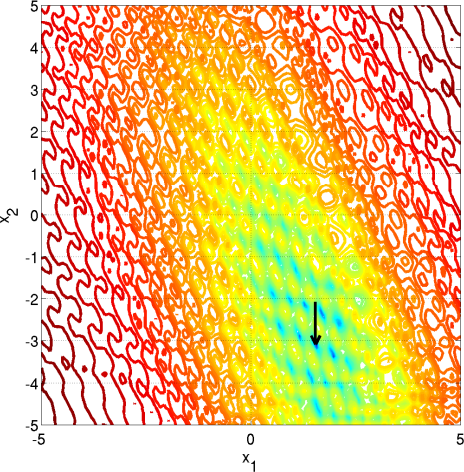
\includegraphics[width=.45\textwidth]{img/15a.png} 
}
\end{figure}

\subsection{Funkcja numer 16 - Weierstrassa}

Funkcja 16 jest obrócona w stosunku do oryginalnej funkcji Weierstrassa. 
Posiada powtarzalny, ale bardzo wyboisty przebieg oraz więcej niż jedno optimum globalne. Właściwości:
\begin{itemize}
 \item Lokalnie nieregularna.
 \item Brak unikalnego optimum globalnego.
\end{itemize} 

\begin{figure}[H]
\centering
\mbox{
\includegraphics[width=.45\textwidth]{img/16.png} \quad
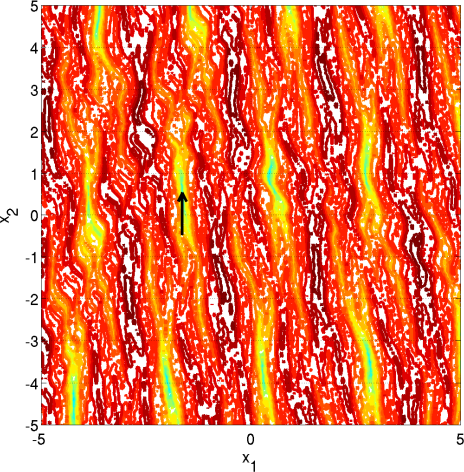
\includegraphics[width=.45\textwidth]{img/16a.png} 
}
\end{figure}

\subsection{Funkcja numer 19 - Griewanka-Rosenbrocka}

Funkcja 19 to złożenie funkcji Griewanka oraz Rosenbrocka, o ogromnej liczbie ekstremów lokalnych.

\begin{figure}[H]
\centering
\mbox{
\includegraphics[width=.45\textwidth]{img/19.png} \quad
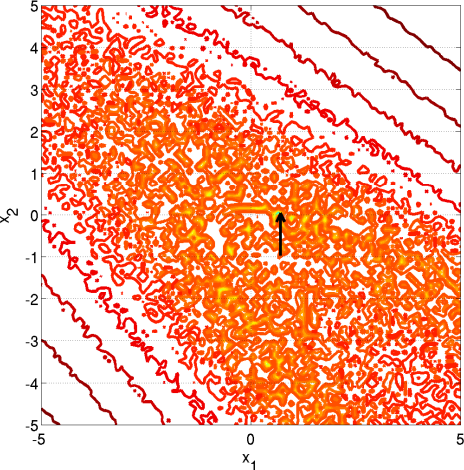
\includegraphics[width=.45\textwidth]{img/19a.png} 
}
\end{figure}

\subsection{Funkcja numer 20 - Schwefela}

Najlepsze $2^D$ minimów lokalnych jest położonych stosunkowo blisko narożników atrakcyjnej hiperpłaszczyzny. Właściwości:
\begin{itemize}
 \item Częściowo separowalna.
 \item Charakterystyczna, obrócona struktura.
 \item Atrakcyjne obszary przeszukiwań znajdują się w narożnikach hiperpłaszczyzny.
\end{itemize} 

\begin{figure}[H]
\centering
\mbox{
\includegraphics[width=.45\textwidth]{img/20.png} \quad
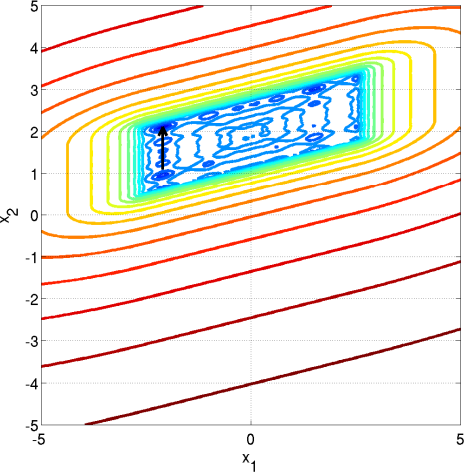
\includegraphics[width=.45\textwidth]{img/20a.png} 
}
\end{figure}

\subsection{Funkcja numer 21 - dołki gaussowskie Gallaghera 101-me}

Funkcja posiada 101 ekstremów lokalnych, których położenie oraz wielkość są losowe i~niezależne od siebie.
Właściwości:
\begin{itemize}
 \item Wskaźnik uwarunkowania wynosi około 30.
 \item Analizowanie wyników na tej funkcji pomaga odpowiedź na następujące pytanie: Czy przeszukiwanie jest efektywne, gdy funkcja celu
nie ma żadnej globalnej struktury?
\end{itemize} 

\begin{figure}[H]
\centering
\mbox{
\includegraphics[width=.45\textwidth]{img/21.png} \quad
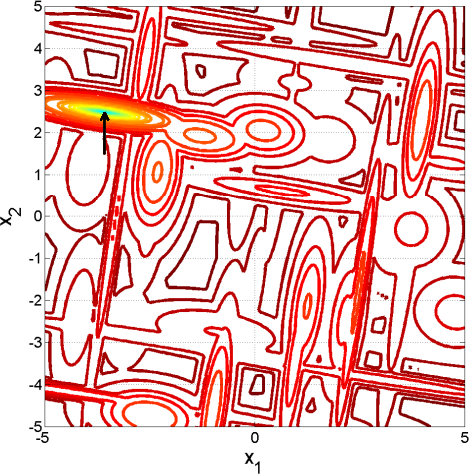
\includegraphics[width=.45\textwidth]{img/21a.png} 
}
\end{figure}

\subsection{Funkcja numer 22 - dołki gaussowskie Gallaghera 21-hi}

Funkcja posiada 21 ekstremów lokalnych, których położenie oraz wielkość są losowe i~niezależne od siebie.
Właściwości:
\begin{itemize}
 \item Wskaźnik uwarunkowania wynosi około 1000.
 \item Analizowanie wyników na tej funkcji pomaga odpowiedź na następujące pytanie: W~porównaniu do funkcji 21, jak 
wysoki wskaźnik uwarunkowania wpływa na efektywność przeszukiwania?
\end{itemize} 

\begin{figure}[H]
\centering
\mbox{
\includegraphics[width=.45\textwidth]{img/22.png} \quad
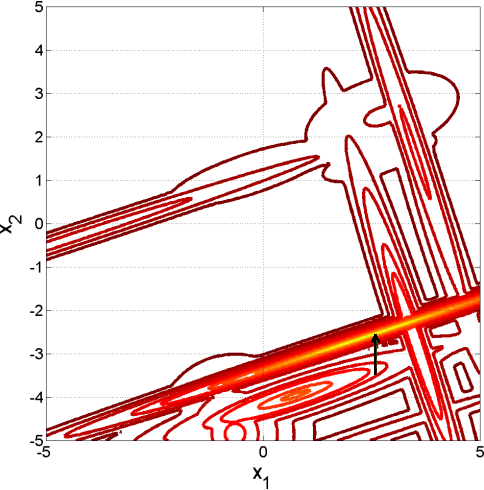
\includegraphics[width=.45\textwidth]{img/22a.png} 
}
\end{figure}

\subsection{Funkcja numer 24 - Lunaceka}

Funkcja Lunaceka jest również nazywana podwójnym Rastriginem (bi-Rastrigin). Funkcja ta ma dużą liczbę ekstremów lokalnych. 
Na jej wykresie można zauważyć dwa charekterystyczne dołki. Żeby znaleźć optimum, algorytm musi najpierw poprawnie wybrać dołek,
a następnie dokładnie przeszukać multimodalną przestrzeń wewnątrz niego. Funkcja została skonstruowana w taki sposób, aby zmylić
niektóre algorytmy ewolucyjne z dużym rozmiarem populacji. Dołek z optimum lokalnym stanowi około 70\% całej przestrzeni przeszukiwań.
Analiza wyników na tej funkcji pomaga odpowiedzieć na następujące pytanie:
Czy przeszukiwanie może mieć charakter lokalny w skali globalnej oraz charakter globalny w skali lokalnej?

\begin{figure}[H]
\centering
\mbox{
\includegraphics[width=.45\textwidth]{img/24.png} \quad
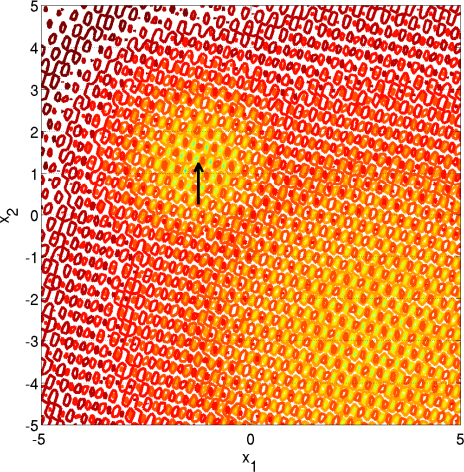
\includegraphics[width=.45\textwidth]{img/24a.png} 
}
\end{figure}

\section{Parametry}

Dla funkcji o małej liczbie wymiarów trudno dostrzec różnicę pomiędzy algorytmami. Im wyższy wymiar,
tym trudniejszy problem i dłuższy czas obliczeń, ale różnice pomiędzy algorytmami stają się bardziej 
widoczne. Dlatego liczba wymiarów $D$ w testach wynosiła 10, 20, 40 oraz 80. 

W niektórych przypadkach znalezienie minimum trwałoby zbyt długo. Dlatego zastosowano kryterium stopu,
jakim jest ograniczenie na maksymalną liczbę wywołań funkcji oceny ($FEs$), wynoszącą $10^5D$, 
zgodnie z \cite{setup}. Rozmiar populacji $n$ dla każdego algorytmu był stały i wynosił $10D$. 
Jeśli algorytm nie znajdował 
minimum, wówczas w jednym uruchomieniu, na jednej funkcji, generował $\frac{FEs}{n} = 10^4$ pokoleń.
Początkowa populacja była inicjalizowana zgodnie z rozkładem jednostajnym w obszarze przeszukiwań tzn.
w hipersześcianie $[-5; 5]^D$. Punkty, które w czasie optymalizacji wyjdą poza obszar
przeszukiwań, nie są naprawiane. Zewnętrzna funkcja kary opisana w rodziale \ref{sec:zestaw}
zapobiega znacznemu oddalaniu się punktów od interesującego obszaru.

Ze wzlędu na losowość procesu optymalizacji, na każdej funkcji algorytm był niezależnie uruchamiany 15 razy.
Z każdego uruchomienia zapisywany był 
najlepszy wynik. Współczynnik skalujący algorytmu DE/rand/1 ($F$) wynosił $0,9$. 
W każdym z algorytmów zostało wykorzystane krzyżowanie wymieniające (DE/*/k/bin) z
prawdopodobieństwem krzyżowania $p_c = 0,9$.

\section{Implementacja}

Zestaw BBOB2013 dostarcza implementację wszystkich funkcji testowych w języku C. Funkcje te obliczane
są miliardy razy podczas eksperymentów, dlatego ważne jest, żeby wykonywały się jak najszybciej.
Procedura testująca oraz badane algorytmy zostały zaimplementowane w 
Javie, ze względu na udogodnienia związane z programowaniem obiektowym, przy pomijalnym spadku 
wydajności. Procedura testująca wywołuje funkcje napisane w~C~dzięki Java Native Interface (JNI).
Do automatyzacji testów oraz przetwarzania wyników zostały napisane skrypty w sh 
(języku powłoki Bourne'a) oraz języku~R. Do przeprowadzenia testów istotności statystycznej Wilcoxona 
użyto funkcji \texttt{wilcox.test} z pakietu \texttt{stats} języka R. Dystrybuanty empiryczne
zostały obliczone dzięki funkcji \texttt{ecdf} (ang. empirical cumulative distribution function),
pochodzącej z tego samego pakietu.

Poprawność implementacji algorytmów w Javie została zweryfikowana dzięki testom macierzy kowariancji
populacji. Zbadano wartości macierzy po pierwszej mutacji, uśrednione z~10000 niezależnych uruchomień. 
Średnie wartości macierzy kowariancji były takie same dla wszystkich badanych algorytmów, zgodnie z 
założeniami teoretycznymi. Uśrednioną macierz kowariancji populacji przedstawia tabela 
\ref{table:cov_matrix}. 

\begin{table}[H]
\centering
\begin{tabular}{ c c c c c c c c c c }
21,36 & 0,02 & 0,01 & -0,04 & 0,06 & -0,01 & -0,03 & -0,02 & -0,01 & 0,03 \\
0,02 & 21,37 & 0,00 & 0,01 & -0,01 & 0,02 & 0,03 & 0,02 & 0,03 & 0,00 \\
0,01 & 0,00 & 21,40 & -0,01 & -0,03 & -0,03 & -0,09 & 0,04 & 0,01 & -0,02 \\
-0,04 & 0,01 & -0,01 & 21,37 & 0,02 & 0,00 & 0,02 & 0,07 & 0,03 & -0,03 \\
0,06 & -0,01 & -0,03 & 0,02 & 21,43 & -0,00 & 0,02 & 0,01 & -0,01 & 0,01 \\
-0,01 & 0,02 & -0,03 & 0,00 & -0,00 & 21,41 & -0,00 & -0,01 & 0,02 & -0,01 \\
-0,03 & 0,03 & -0,09 & 0,02 & 0,02 & -0,00 & 21,38 & 0,04 & 0,05 & -0,01 \\
-0,02 & 0,02 & 0,04 & 0,07 & 0,01 & -0,01 & 0,04 & 21,40 & -0,05 & 0,04 \\
-0,01 & 0,03 & 0,01 & 0,03 & -0,01 &  0,02 & 0,05 & -0,05 & 21,39 & 0,02 \\
0,03 & 0,00 & -0,02 & -0,03 & 0,01 & -0,01 & -0,01 &  0,04 & 0,02 & 21,37 \\
\end{tabular}
\caption{Uśredniona macierz kowariancji dla 10-wymiarowej funkcji numer 15.}
\label{table:cov_matrix}
\end{table}

Wszystkie funkcje użyte do testów są nieseparowalne liniowo, w szczególności funkcja 15.
Dlatego wartości macierzy kowariancji populacji poza główną przekątną są bliskie 0. Oznacza to,
iż korelacja liniowa Pearsona pomiędzy wartościami różnych cech praktycznie nie występuje, wymiary
są niezależne od siebie. Z kolei wartość bliska 21,4 powtarzająca się na głównej przekątnej 
oznacza taką samą wariancję wartości w każdym z wymiarów, tzn. dla każdej cechy osobnika.
Wartość ta jest identyczna dla wszystkich algorytmów, dzięki odpowiednim współczynnikom skalującym
$F$ wyprowadzonych wcześniej w tej pracy. Dzięki takiej samej macierzy kowariancji algorytmy
mają takie same warunki i wyniki przez nie zwracane zależą tylko od sposobu mutacji, nie od jej
zasięgu.

\section{Porównywanie wyników}

Duża liczba wariantów algorytmów wymaga systematycznego i wiarygodnego sposobu porównywania
i prezentacji wyników. Testy istotności statystycznej pozwalają w szybki sposób rozstrzygnąć czy 
wyniki osiągane przez dwa algorytmy są od siebie istotnie różne. Dystrybuanty empiryczne
pozwalają zorientować się na ile wyniki algorytmów różnią się od siebie. \%~osobników, które
znalazły się poza przestrzenią przeszukiwań, pozwala ocenić czy algorytm dotarł do krawędzi
obszaru przeszukiwań czy pozostawał cały czas w jego wnętrzu.

\subsection{Testy istotności statystycznej}

W tej pracy jako podstawowy sposób porównywania wyników został wykorzystany test 
Wilcoxona dla par obserwacji. Zaproponowany pierwotnie jako test przesunięcia dla dwóch równolicznych 
próbek przez Franka Wilcoxona w 1945, uogólniony następnie przez Manna i Whitneya w 1947
dla przypadku różnolicznych próbek \cite{mann}. Test Wilcoxona to nieparametryczna alternatywa dla testu t-Studenta w 
przypadku dwóch równolicznych próbek. Test t-Studenta sprawdza hipotezę zerową o równości
średnich arytmetycznych w odpowiadających im populacjach, natomiast test Wilcoxona
weryfikuje równość median. Średnia jest wrażliwa na wartości odstające,
natomiast mediana nie. Ponadto, test t-Studenta jest parametryczny, to znaczy zakłada pewien rozkład
wartości z badanej próby. Test Wilcoxona jest nieparametryczny, to znaczy,
nie zakłada nic na temat rozkładu badanych wartości i dlatego został wybrany.

$n$ par obserwacji pochodzi z dwóch zbiorów. Pierwszy element pary pochodzi ze zbioru pierwszego, drugi element pary 
ze zbioru drugiego. W tej pracy $n=15$,
ponieważ liczba niezależnych uruchomień algorytmu wynosiła 15. Pierwszy zbiór odpowiada algorytmowi A i zawiera
liczby $x_1, x_2, \dots, x_{n}$, drugi -- algorytmowi B i zawiera liczby $y_1, y_2, \dots, y_{n}$. 
Liczby w zbiorach oznaczają odległość najlepszego osobnika uzyskanego w jednym uruchomieniu
od minimum optymalizowanej funkcji. Zostały spełnione wszystkie założenia dla testu Wilcoxona:

\begin{enumerate}
 \item Wartości $x_i$ i $y_i$ są parowane w sposób losowo niezależny od siebie. 
 \item Wartości $x_i$ i $y_i$ pochodzą z populacji o rozkładzie ciągłym.
 \item Wartości $x_i$ i $y_i$ można porównywać ze sobą, jednoznacznie stwierdzając która jest większa, mniejsza,
bądź równa.
\end{enumerate}

Testowana hipoteza zerowa $H_0$ brzmi: ,,różnica pomiędzy medianami ze zbioru A i B wynosi zero''.
Hipoteza alternatywna $H_1$ brzmi ,,różnica pomiędzy medianami ze zbioru A i B jest różna od zera''.
Test Wilcoxona przebiega następująco:

\begin{enumerate}
 \item Obliczenie różnic $d_i = y_i - x_i$.
 \item Usunięcie par dla których $d_i = 0$. Niech $N \leq n$ oznacza liczbę pozostałych par.
 \item Posortowanie rosnąco wartości bezwględnych różnic $|d_i|$.
 \item Rangowanie posortowanego zbioru rangami $R_i$, poczynając od rangi równej 1. 
 \item Obliczenie statystyki $W = |\sum\limits_{i=1}^{N} \sgn(d_i)R_i|$.
 \item Rozkład $W$ zbiega do rozkładu normalnego wraz ze wzrostem $N$. Obliczane jest
 $p = \frac{W - 0,5}{\sigma_W}$, gdzie $\sigma_W = \sqrt{\frac{N(N+1)(2N+1)}{6}}.$ 
 \item Jeśli $z > z_{critical}$, hipoteza $H_0$ jest odrzucana, w przeciwnym przypadku -- przyjmowana. 
Wartości $z_{critical}$ zależą od przyjętego poziomu ufności. 
W tej pracy poziom ufności wynosił $0,05$, co odpowiada $z_{critical}=1,96$ \cite{lowry}.  
\end{enumerate}

Jeśli test nie pozwalał na odrzucenie hipotezy zerowej, uznawano, że wyniki porównywanych algorytmów
nie są istotnie różne od siebie. W notacji stosowanej w tabelach brak statystycznej różnicy oznaczono
znakiem $\cdotp$.
Jeśli test odrzucał hipotezę zerową, uznawano, że algorytmy A i B dają różne wyniki.
Wówczas porówywane były mediany obu zbiorów. Algorytm, którego mediana wyników była niższa,
uznawany był za lepszy i oznaczany znakiem +. Algorytm istotnie gorszy był oznaczany znakiem --.

\subsection{Dystrybuanty empiryczne}

W celu relatywnego porównania wyników osiąganych przez algorytmy, 
wykreślono dystrybuanty empiryczne najlepszych wyników z każdego uruchomienia 
dla wszystkich algorytmów na jednej funkcji. Najlepszym wynikiem była odległość najlepszego 
osobnika uzyskanego w jednym uruchomieniu od minimum optymalizowanej funkcji. Oś x wykresu
odpowiada wartościom najlepszych wyników osiąganych przez algorytmy. Oś y odpowiada natomiast 
estymowanemu prawdopodobieństwu, z jakim algorytm osiąga dany wynik. Dystrybuanty pozwalają również
określić jak bliskie minimum było najlepsze znalezione przez algorytm rozwiązanie.

\subsection{\% osobników poza obszarem przeszukiwań}

W każdym uruchomieniu zliczana była liczba osobników, których jakakolwiek współrzędna wykraczała poza
obszar przeszukiwań zdefiniowany jako $[-5; 5]^D$. Następnie obliczany był stosunek liczby 
osobników spoza obszaru przeszukiwań do liczby wszystkich wygenerowanych osobników. Jeśli algorytm
nie znajdywał minimum, wówczas liczba wszystkich generowanych osobników była równa maksymalnej liczbie
populacji razy $n$, czyli $\frac{FEs}{n} \cdot n = FEs = 10^5D$. W~przypadku nie odnalezienia minimum, 
1\% w 10 wymiarach oznacza, że 
w trakcie optymalizacji algorytm wygenerował i ocenił 10000 osobników, 
które na pewno nie mogły być rozwiązaniami optymalnymi,
ponieważ leżały poza obszarem przeszukiwań. Dla jednego algorytmu na jednej funkcji, \% osobników
poza obszarem przeszukiwań uśredniano z 15 niezależnych uruchomień.

\chapter{Wyniki eksperymentów}

\section{10 wymiarów}

\begin{table}[H]
\centering
\begin{tabular}{ l | c | c | c | c | c | c | c }
algorytm         &f15& 16& 19& 20& 21& 22& 24 \\ \hline
DE/rand/2	 & + & + & $\cdot$ & + & $\cdot$ & $\cdot$ & $\cdot$ \\
DE/rand/6	 & + & + & $\cdot$ & + & $\cdot$ & $\cdot$ & $\cdot$ \\
DE/rand/$\infty$	 & + & + & $\cdot$ & + & $\cdot$ & $\cdot$ & $\cdot$ \\
DE/best/1	 & + & + & + & + & + & + & + \\
DE/best/2	 & + & + & $\cdot$ & + & $\cdot$ & $\cdot$ & $\cdot$ \\
DE/best/6	 & + & + & + & + & $\cdot$ & $\cdot$ & + \\
DE/best/$\infty$	 & + & + & + & + & + & $\cdot$ & + \\
DE/mid/1	 & -- & + & -- & + & $\cdot$ & $\cdot$ & -- \\
DE/mid/2	 & + & + & $\cdot$ & + & + & $\cdot$ & $\cdot$ \\
DE/mid/6	 & + & + & $\cdot$ & + & $\cdot$ & $\cdot$ & $\cdot$ \\
DE/mid/$\infty$	 & + & + & $\cdot$ & + & $\cdot$ & $\cdot$ & $\cdot$ \\
\end{tabular}
\caption{Porównanie DE/rand/1 do reszty algorytmów}
\end{table}

\begin{table}[H]
\centering
\begin{tabular}{ l | c | c | c | c | c | c | c }
algorytm         &f15& 16& 19& 20& 21& 22& 24 \\ \hline
DE/rand/1	 & -- & -- & -- & -- & -- & -- & -- \\
DE/rand/2	 & -- & $\cdot$ & -- & + & -- & -- & -- \\
DE/rand/6	 & -- & $\cdot$ & -- & + & -- & -- & -- \\
DE/rand/$\infty$	 & -- & $\cdot$ & -- & + & -- & -- & -- \\
DE/best/2	 & -- & -- & -- & -- & -- & -- & -- \\
DE/best/6	 & $\cdot$ & + & -- & + & -- & -- & -- \\
DE/best/$\infty$	 & $\cdot$ & + & -- & + & $\cdot$ & -- & -- \\
DE/mid/1	 & -- & $\cdot$ & -- & + & -- & -- & -- \\
DE/mid/2	 & -- & $\cdot$ & -- & + & $\cdot$ & -- & -- \\
DE/mid/6	 & -- & $\cdot$ & -- & + & -- & -- & -- \\
DE/mid/$\infty$	 & -- & $\cdot$ & -- & + & -- & -- & -- \\
\end{tabular}
\caption{Porównanie DE/best/1 do reszty algorytmów}
\end{table}

\begin{table}[H]
\centering
\begin{tabular}{ l | c | c | c | c | c | c | c }
algorytm         &f15& 16& 19& 20& 21& 22& 24 \\ \hline
DE/rand/1	 & + & -- & + & -- & $\cdot$ & $\cdot$ & + \\
DE/rand/2	 & + & + & + & -- & $\cdot$ & $\cdot$ & + \\
DE/rand/6	 & + & + & + & $\cdot$ & -- & $\cdot$ & + \\
DE/rand/$\infty$	 & + & $\cdot$ & + & $\cdot$ & $\cdot$ & $\cdot$ & + \\
DE/best/1	 & + & $\cdot$ & + & -- & + & + & + \\
DE/best/2	 & + & $\cdot$ & + & -- & $\cdot$ & $\cdot$ & + \\
DE/best/6	 & + & + & + & + & $\cdot$ & $\cdot$ & + \\
DE/best/$\infty$	 & + & + & + & + & + & $\cdot$ & + \\
DE/mid/2	 & + & + & + & $\cdot$ & $\cdot$ & $\cdot$ & + \\
DE/mid/6	 & + & + & + & $\cdot$ & $\cdot$ & $\cdot$ & + \\
DE/mid/$\infty$	 & + & + & + & $\cdot$ & $\cdot$ & $\cdot$ & + \\
\end{tabular}
\caption{Porównanie DE/mid/1 do reszty algorytmów}
\end{table}

\begin{table}[H]
\centering
\begin{tabular}{ l | c | c | c | c | c | c | c }
algorytm         &f15& 16& 19& 20& 21& 22& 24 \\ \hline
DE/rand/1	 & 1 & 30 & 7 & 0 & 1 & 1 & 0 \\
DE/rand/2	 & 8 & 43 & 9 & 0 & 5 & 3 & 0 \\
DE/rand/6	 & 9 & 43 & 8 & 0 & 9 & 5 & 0 \\
DE/rand/$\infty$ & 9 & 43 & 10 & 0 & 10 & 7 & 0 \\
DE/best/1	 & 8 & 18 & 5 & 0 & 0 & 3 & 0 \\
DE/best/2	 & 6 & 19 & 6 & 0 & 2 & 2 & 0 \\
DE/best/6	 & 7 & 22 & 7 & 0 & 7 & 7 & 0 \\
DE/best/$\infty$ & 7 & 22 & 7 & 0 & 10 & 7 & 0 \\
DE/mid/1         & 0 & 27 & 0 & 0 & 1 & 1 & 0 \\
DE/mid/2	 & 5 & 42 & 10 & 0 & 12 & 16 & 0 \\
DE/mid/6	 & 8 & 43 & 11 & 0 & 9 & 6 & 0 \\
DE/mid/$\infty$	 & 9 & 43 & 11 & 0 & 11 & 6 & 0 \\ \hline
średnia          & 6 & 33 & 8 & 0 & 6 & 5 & 0 \\              
\end{tabular}
\caption{Średni \% osobników poza obszarem przeszukiwań}
\end{table}

\begin{figure}[H]
\centering
\mbox{
\includegraphics[width=.45\textwidth]{../pngs/10/15.png} \quad
\includegraphics[width=.45\textwidth]{../pngs/10/16.png} 
}
\end{figure}

\begin{figure}[H]
\centering
\mbox{
\includegraphics[width=.45\textwidth]{../pngs/10/19.png} \quad
\includegraphics[width=.45\textwidth]{../pngs/10/20.png} 
}
\end{figure}

\begin{figure}[H]
\centering
\mbox{
\includegraphics[width=.45\textwidth]{../pngs/10/21.png} \quad
\includegraphics[width=.45\textwidth]{../pngs/10/22.png} 
}
\end{figure}

\begin{figure}[H]
\centering
\mbox{
\includegraphics[width=.45\textwidth]{../pngs/10/24.png}
}
\end{figure}

\section{20 wymiarów}

\begin{table}[H]
\centering
\begin{tabular}{ l | c | c | c | c | c | c | c }
algorytm         &f15& 16& 19& 20& 21& 22& 24 \\ \hline
DE/rand/2	 & + & + & + & + & $\cdot$ & $\cdot$ & + \\
DE/rand/6	 & + & + & + & + & + & $\cdot$ & + \\
DE/rand/$\infty$	 & + & + & + & + & + & $\cdot$ & + \\
DE/best/1	 & + & + & + & + & + & + & + \\
DE/best/2	 & + & + & + & + & + & + & + \\
DE/best/6	 & + & + & + & + & + & + & + \\
DE/best/$\infty$	 & + & + & + & + & + & + & + \\
DE/mid/1	 & $\cdot$ & + & $\cdot$ & + & $\cdot$ & $\cdot$ & + \\
DE/mid/2	 & + & + & + & + & + & $\cdot$ & + \\
DE/mid/6	 & + & + & + & + & + & $\cdot$ & + \\
DE/mid/$\infty$	 & + & + & + & + & + & $\cdot$ & + \\
\end{tabular}
\caption{Porównanie DE/rand/1 do reszty algorytmów}
\end{table}

\begin{table}[H]
\centering
\begin{tabular}{ l | c | c | c | c | c | c | c }
algorytm         &f15& 16& 19& 20& 21& 22& 24 \\ \hline
DE/rand/1	 & -- & -- & -- & -- & -- & -- & -- \\
DE/rand/2	 & $\cdot$ & + & $\cdot$ & + & -- & -- & -- \\
DE/rand/6	 & + & + & $\cdot$ & + & $\cdot$ & -- & -- \\
DE/rand/$\infty$	 & + & + & $\cdot$ & + & $\cdot$ & -- & -- \\
DE/best/2	 & + & + & + & + & $\cdot$ & $\cdot$ & + \\
DE/best/6	 & + & + & + & + & + & + & + \\
DE/best/$\infty$	 & + & + & + & + & + & + & + \\
DE/mid/1	 & -- & + & -- & + & -- & -- & -- \\
DE/mid/2	 & -- & + & -- & + & $\cdot$ & -- & -- \\
DE/mid/6	 & $\cdot$ & + & $\cdot$ & + & $\cdot$ & -- & -- \\
DE/mid/$\infty$	 & $\cdot$ & + & $\cdot$ & + & $\cdot$ & -- & -- \\
\end{tabular}
\caption{Porównanie DE/best/1 do reszty algorytmów}
\end{table}

\begin{table}[H]
\centering
\begin{tabular}{ l | c | c | c | c | c | c | c }
algorytm         &f15& 16& 19& 20& 21& 22& 24 \\ \hline
DE/rand/1	 & $\cdot$ & -- & $\cdot$ & -- & $\cdot$ & $\cdot$ & -- \\
DE/rand/2	 & + & + & + & $\cdot$ & $\cdot$ & $\cdot$ & + \\
DE/rand/6	 & + & + & + & + & + & $\cdot$ & + \\
DE/rand/$\infty$	 & + & + & + & $\cdot$ & + & $\cdot$ & + \\
DE/best/1	 & + & -- & + & -- & + & + & + \\
DE/best/2	 & + & + & + & + & + & + & + \\
DE/best/6	 & + & + & + & + & + & + & + \\
DE/best/$\infty$	 & + & + & + & + & + & + & + \\
DE/mid/2	 & + & + & + & $\cdot$ & + & $\cdot$ & + \\
DE/mid/6	 & + & + & + & $\cdot$ & + & $\cdot$ & + \\
DE/mid/$\infty$	 & + & + & + & $\cdot$ & + & $\cdot$ & + \\
\end{tabular}
\caption{Porównanie DE/mid/1 do reszty algorytmów}
\end{table}

\begin{table}[H]
\centering
\begin{tabular}{ l | c | c | c | c | c | c | c }
algorytm         &f15& 16& 19& 20& 21& 22& 24 \\ \hline
DE/rand/1	 & 12 & 38 & 2 & 2 & 4 & 5 & 0   \\
DE/rand/2	 & 30 & 47 & 13 & 5 & 23 & 20 & 0  \\
DE/rand/6	 & 33 & 47 & 16 & 5 & 31 & 27 & 0     \\
DE/rand/$\infty$ & 34 & 47 & 18 & 5 & 33 & 28 & 0  \\
DE/best/1	 & 8 & 21 & 1 & 0 & 1 & 2 & 0      \\
DE/best/2	 & 21 & 22 & 11 & 8 & 15 & 16 & 0   \\
DE/best/6	 & 23 & 21 & 15 & 13 & 15 & 15 & 1      \\
DE/best/$\infty$ & 23 & 21 & 14 & 12 & 15 & 16 & 1 \\
DE/mid/1         & 3 & 42 & 0 & 0 & 0 & 0 & 0  \\
DE/mid/2	 & 23 & 47 & 9 & 3 & 25 & 18 & 0  \\
DE/mid/6	 & 32 & 47 & 18 & 5 & 31 & 26 & 0  \\
DE/mid/$\infty$	 & 32 & 47 & 17 & 4 & 32 & 25 & 0 \\ \hline
średnia          & 23 & 37 & 11 & 5 & 19 & 17 & 0 \\  
\end{tabular}
\caption{Średni \% osobników poza obszarem przeszukiwań}
\end{table}

\begin{figure}[H]
\centering
\mbox{
\includegraphics[width=.45\textwidth]{../pngs/20/15.png} \quad
\includegraphics[width=.45\textwidth]{../pngs/20/16.png} 
}
\end{figure}

\begin{figure}[H]
\centering
\mbox{
\includegraphics[width=.45\textwidth]{../pngs/20/19.png} \quad
\includegraphics[width=.45\textwidth]{../pngs/20/20.png} 
}
\end{figure}

\begin{figure}[H]
\centering
\mbox{
\includegraphics[width=.45\textwidth]{../pngs/20/21.png} \quad
\includegraphics[width=.45\textwidth]{../pngs/20/22.png} 
}
\end{figure}

\begin{figure}[H]
\centering
\mbox{
\includegraphics[width=.45\textwidth]{../pngs/20/24.png} \quad
}
\end{figure}

\section{40 wymiarów}

\begin{table}[H]
\centering
\begin{tabular}{ l | c | c | c | c | c | c | c }
algorytm         &f15& 16& 19& 20& 21& 22& 24 \\ \hline
DE/rand/2	 & + & + & + & + & + & + & + \\
DE/rand/6	 & + & + & + & + & + & + & + \\
DE/rand/$\infty$	 & + & + & + & + & + & + & + \\
DE/best/1	 & + & -- & + & + & + & + & + \\
DE/best/2	 & + & + & + & + & + & + & + \\
DE/best/6	 & + & + & + & + & + & + & + \\
DE/best/$\infty$	 & + & + & + & + & + & + & + \\
DE/mid/1	 & -- & $\cdot$ & -- & + & $\cdot$ & $\cdot$ & -- \\
DE/mid/2	 & + & + & + & + & + & + & + \\
DE/mid/6	 & + & + & + & + & + & + & + \\
DE/mid/$\infty$	 & + & + & + & + & + & + & + \\
\end{tabular}
\caption{Porównanie DE/rand/1 do reszty algorytmów}
\end{table}

\begin{table}[H]
\centering
\begin{tabular}{ l | c | c | c | c | c | c | c }
algorytm         &f15& 16& 19& 20& 21& 22& 24 \\ \hline
DE/rand/1	 & -- & + & -- & -- & -- & -- & -- \\
DE/rand/2	 & + & + & + & + & + & + & + \\
DE/rand/6	 & + & + & + & + & + & + & + \\
DE/rand/$\infty$	 & + & + & + & + & + & + & + \\
DE/best/2	 & + & + & + & + & + & + & + \\
DE/best/6	 & + & + & + & + & + & + & + \\
DE/best/$\infty$	 & + & + & + & + & + & + & + \\
DE/mid/1	 & -- & + & -- & -- & -- & -- & -- \\
DE/mid/2	 & -- & + & $\cdot$ & -- & $\cdot$ & $\cdot$ & -- \\
DE/mid/6	 & + & + & + & + & + & + & + \\
DE/mid/$\infty$	 & + & + & + & + & + & + & + \\
\end{tabular}
\caption{Porównanie DE/best/1 do reszty algorytmów}
\end{table}

\begin{table}[H]
\centering
\begin{tabular}{ l | c | c | c | c | c | c | c }
algorytm         &f15& 16& 19& 20& 21& 22& 24 \\ \hline
DE/rand/1	 & + & $\cdot$ & + & -- & $\cdot$ & $\cdot$ & + \\
DE/rand/2	 & + & + & + & + & + & + & + \\
DE/rand/6	 & + & + & + & + & + & + & + \\
DE/rand/$\infty$	 & + & + & + & + & + & + & + \\
DE/best/1	 & + & -- & + & + & + & + & + \\
DE/best/2	 & + & + & + & + & + & + & + \\
DE/best/6	 & + & + & + & + & + & + & + \\
DE/best/$\infty$	 & + & + & + & + & + & + & + \\
DE/mid/2	 & + & + & + & + & + & + & + \\
DE/mid/6	 & + & + & + & + & + & + & + \\
DE/mid/$\infty$	 & + & + & + & + & + & + & + \\
\end{tabular}
\caption{Porównanie DE/mid/1 do reszty algorytmów}
\end{table}

\begin{table}[H]
\centering
\begin{tabular}{ l | c | c | c | c | c | c | c }
algorytm         &f15& 16& 19& 20& 21& 22& 24 \\ \hline
DE/rand/1	 & 31 & 42 & 3 & 6 & 17 & 16 & 0   \\
DE/rand/2	 & 47 & 42 & 35 & 45 & 14 & 12 & 2   \\
DE/rand/6	 & 44 & 41 & 35 & 43 & 4 & 3 & 0      \\
DE/rand/$\infty$ & 43 & 40 & 33 & 42 & 3 & 2 & 0   \\
DE/best/1	 & 24 & 19 & 0 & 1 & 4 & 11 & 0    \\
DE/best/2	 & 20 & 18 & 10 & 19 & 0 & 0 & 0    \\
DE/best/6	 & 17 & 16 & 6 & 15 & 0 & 0 & 0      \\
DE/best/$\infty$ & 16 & 16 & 6 & 15 & 0 & 0 & 0  \\
DE/mid/1         & 7 & 45 & 0 & 0 & 1 & 1 & 0  \\
DE/mid/2	 & 46 & 43 & 17 & 26 & 26 & 25 & 2   \\
DE/mid/6	 & 44 & 40 & 35 & 43 & 4 & 3 & 0     \\
DE/mid/$\infty$	 & 43 & 38 & 35 & 44 & 5 & 3 & 0    \\ \hline
średnia          & 32 & 33 & 18 & 25 & 7 & 6 & 0 \\  
\end{tabular}
\caption{Średni \% osobników poza obszarem przeszukiwań}
\end{table}

\begin{figure}[H]
\centering
\mbox{
\includegraphics[width=.45\textwidth]{../pngs/40/15.png} \quad
\includegraphics[width=.45\textwidth]{../pngs/40/16.png} 
}
\end{figure}

\begin{figure}[H]
\centering
\mbox{
\includegraphics[width=.45\textwidth]{../pngs/40/19.png} \quad
\includegraphics[width=.45\textwidth]{../pngs/40/20.png} 
}
\end{figure}

\begin{figure}[H]
\centering
\mbox{
\includegraphics[width=.45\textwidth]{../pngs/40/21.png} \quad
\includegraphics[width=.45\textwidth]{../pngs/40/22.png} 
}
\end{figure}

\begin{figure}[H]
\centering
\mbox{
\includegraphics[width=.45\textwidth]{../pngs/40/24.png} \quad
}
\end{figure}

\section{80 wymiarów}

\begin{table}[H]
\centering
\begin{tabular}{ l | c | c | c | c | c | c | c }
algorytm         &f15& 16& 19& 20& 21& 22& 24 \\ \hline
DE/rand/2	 & + & + & + & + & + & + & + \\
DE/rand/6	 & + & + & + & + & + & + & + \\
DE/rand/$\infty$	 & + & + & + & + & + & + & + \\
DE/best/1	 & + & -- & + & + & + & $\cdot$ & + \\
DE/best/2	 & + & + & + & + & + & + & + \\
DE/best/6	 & + & + & + & + & + & + & + \\
DE/best/$\infty$	 & + & + & + & + & + & + & + \\
DE/mid/1	 & -- & $\cdot$ & -- & -- & -- & -- & -- \\
DE/mid/2	 & + & + & + & + & + & + & + \\
DE/mid/6	 & + & + & + & + & + & + & + \\
DE/mid/$\infty$	 & + & + & + & + & + & + & + \\
\end{tabular}
\caption{Porównanie DE/rand/1 do reszty algorytmów}
\end{table}

\begin{table}[H]
\centering
\begin{tabular}{ l | c | c | c | c | c | c | c }
algorytm         &f15& 16& 19& 20& 21& 22& 24 \\ \hline
DE/rand/1	 & -- & + & -- & -- & -- & $\cdot$ & -- \\
DE/rand/2	 & + & + & + & + & + & + & + \\
DE/rand/6	 & + & + & + & + & + & + & + \\
DE/rand/$\infty$	 & + & + & + & + & + & + & + \\
DE/best/2	 & + & + & + & + & + & + & + \\
DE/best/6	 & + & + & + & + & + & + & + \\
DE/best/$\infty$	 & + & + & + & + & + & + & + \\
DE/mid/1	 & -- & + & -- & -- & -- & -- & -- \\
DE/mid/2	 & + & + & -- & -- & + & + & + \\
DE/mid/6	 & + & + & + & + & + & + & + \\
DE/mid/$\infty$	 & + & + & + & + & + & + & + \\

\end{tabular}
\caption{Porównanie DE/best/1 do reszty algorytmów}
\end{table}

\begin{table}[H]
\centering
\begin{tabular}{ l | c | c | c | c | c | c | c }
algorytm         &f15& 16& 19& 20& 21& 22& 24 \\ \hline
DE/rand/1	 & + & $\cdot$ & + & + & + & + & + \\
DE/rand/2	 & + & + & + & + & + & + & + \\
DE/rand/6	 & + & + & + & + & + & + & + \\
DE/rand/$\infty$	 & + & + & + & + & + & + & + \\
DE/best/1	 & + & -- & + & + & + & + & + \\
DE/best/2	 & + & + & + & + & + & + & + \\
DE/best/6	 & + & + & + & + & + & + & + \\
DE/best/$\infty$	 & + & + & + & + & + & + & + \\
DE/mid/2	 & + & + & + & + & + & + & + \\
DE/mid/6	 & + & + & + & + & + & + & + \\
DE/mid/$\infty$	 & + & + & + & + & + & + & + \\
\end{tabular}
\caption{Porównanie DE/mid/1 do reszty algorytmów}
\end{table}

\begin{table}[H]
\centering
\begin{tabular}{ l | c | c | c | c | c | c | c }
algorytm         &f15& 16& 19& 20& 21& 22& 24 \\ \hline
DE/rand/1	 & 40 & 39 & 10 & 20 & 16 & 17 & 1    \\
DE/rand/2	 & 39 & 36 & 18 & 32 & 0 & 0 & 0  \\
DE/rand/6	 & 31 & 32 & 4 & 21 & 0 & 0 & 0        \\
DE/rand/$\infty$ & 30 & 30 & 3 & 19 & 0 & 0 & 0     \\
DE/best/1	 & 22 & 20 & 1 & 2 & 11 & 10 & 0   \\
DE/best/2	 & 12 & 14 & 1 & 8 & 0 & 0 & 0     \\
DE/best/6	 & 8 & 11 & 0 & 4 & 0 & 0 & 0        \\
DE/best/$\infty$ & 8 & 9 & 0 & 4 & 0 & 0 & 0      \\
DE/mid/1         & 14 & 46 & 1 & 1 & 2 & 3 & 0   \\
DE/mid/2	 & 45 & 39 & 30 & 40 & 1 & 0 & 0      \\
DE/mid/6	 & 32 & 30 & 4 & 22 & 0 & 0 & 0     \\
DE/mid/$\infty$	 & 28 & 26 & 3 & 19 & 0 & 0 & 0     \\ \hline
średnia          & 26 & 28 & 6 & 16 & 3 & 3 & 0 \\  
\end{tabular}
\caption{Średni \% osobników poza obszarem przeszukiwań}
\end{table}

\begin{figure}[H]
\centering
\mbox{
\includegraphics[width=.45\textwidth]{../pngs/80/15.png} \quad
\includegraphics[width=.45\textwidth]{../pngs/80/16.png} 
}
\end{figure}

\begin{figure}[H]
\centering
\mbox{
\includegraphics[width=.45\textwidth]{../pngs/80/19.png} \quad
\includegraphics[width=.45\textwidth]{../pngs/80/20.png} 
}
\end{figure}

\begin{figure}[H]
\centering
\mbox{
\includegraphics[width=.45\textwidth]{../pngs/80/21.png} \quad
\includegraphics[width=.45\textwidth]{../pngs/80/22.png} 
}
\end{figure}

\begin{figure}[H]
\centering
\mbox{
\includegraphics[width=.45\textwidth]{../pngs/80/24.png} \quad
}
\end{figure}

\chapter{Wnioski}

\section{Wpływ liczby wymiarów na jakość rozwiązań}

Wraz ze wzrostem liczby wymiarów, algorytm DE/mid/1 sprawuje się coraz lepiej.
W~80~wymiarach jednoznacznie wygrywa ze wszystkimi pozostałymi algorytmami na 6~z~7~funkcji testowych.
Jedynie na funkcji numer 16 przegrywa z DE/best/1 oraz remisuje z~DE/rand/1.
W~40~wymiarach prowadzenie DE/mid/1 wygląda podobnie, jedynie różnica w~stosunku do DE/rand/1
jest mniejsza, z którym to wygrywa na 3 funkcjach, remisuje również na 3, a~na 1~przegrywa.
W~20~wymiarach zajmuje drugie miejsce, ustępując DE/rand/1.
W~10~wymiarach było najwięcej remisów, DE/mid/1 był niepokonany na funkcjach numer 15, 19 oraz 24.

\section{Wpływ liczby wymiarów na liczbę osobników poza obszarem przeszukiwań}

Wraz ze wzrostem liczby wymiarów, początkowo średni \% osobników poza obszarem przeszukiwań również 
wzrasta, będąc najwyższy dla 20 lub 40 wymiarów, w zależności od funkcji. Jednak wraz z dalszym
wzrostem liczby wymiarów, \% osobników poza obszarem przeszukiwań spada. 

\begin{table}[H]
\centering
\begin{tabular}{ l | c | c | c | c | c | c | c }
$D$ &f15& 16& 19& 20& 21& 22& 24 \\ \hline
10              & 6 & 33 &  8 &  0 & 6 & 5 & 0 \\
20              & 23 & 37 & 11&  5 & 19 & 17 & 0 \\
40		& 32 & 33 & 18 & 25 & 7 & 6 & 0 \\
80		& 26 & 28 & 6 & 16 & 3 & 3 & 0 \\
\end{tabular}
\caption{Wpływ liczby wymiarów na średni \% osobników poza obszarem przeszukiwań}
\end{table}

\section{Wpływ optymalizowanych funkcji}

Na funkcji 15 oraz 19 zawsze zwyciężał DE/mid/1 -- poza jednym remisem z DE/rand/1 w 20 wymiarach.
\% osobników poza obszarem przeszukiwań na tych funkcjach dla DE/mid/1 zawsze był najniższy.

Funkcja 16 była najgorsza dla DE/mid/1. W 10 i 20 wymiarach, zawsze wygrywał na niej DE/rand/1,
zaś w 40 i 80 wymiarach -- DE/best/1. Spośród trójcy DE/rand/1, DE/best/1, DE/mid/1 
zawsze najniższy \% osobników poza obszarem przeszukiwań miał DE/best/1, potem DE/rand/1, na końcu
DE/mid/1. 

Na funkcji 20 w wymiarach niższych niż 80 zawsze wygrywał DE/rand/1. Dopiero w 80 wymiarze DE/mid/1
objął prowadzenie. DE/mid/1 zawsze miał najniższy \% osobników poza obszarem przesukiwań.

Na funkcji 21 w niższych wymiarach najlepsze wyniki dawał DE/rand/1. W 40 wymiarach wygrał ze 
wszystkimi algorytmami, oprócz DE/mid/1, z którym zremisował. W 80 wymiarach jednak DE/mid/1
okazał się bezkonkurencyjny. DE/mid/1 miał zawsze niższy \% osobników poza obszarem przesukiwań
od DE/rand/1. Mimo, że funkcja 21 nie ma żadnej globalnej struktury, dla DE/mid/1 nie stanowi to 
przeszkody.

Na funkcji 22 w niższych wymiarach sytuacja była remisowa. 
W 40 i 80 wymiarach relacja pomiędzy DE/mid/1 oraz DE/rand/1 jest taka sama jak w przypadku funkcji 21
-- w 40 wymiarach remis, natomiast w 80 zwycięstwo DE/mid/1. \% osobników DE/mid/1 poza obszarem 
przesukiwań cały czas utrzymuje się na niskim poziomie, niemal zawsze najniższym w porównaniu do 
innych algorytmów.
W porównaniu do funkcji 21, wysoki wskaźnik uwarunkowania powoduje mały spadek efektywności
przeszukiwania testowanych algorytmów. Ich kolejność w rankingu jakości zwracanych rozwiązań nie 
zmienia się.

Na funkcji 24 DE/mid/1 przegrał tylko w wymiarze 20 z DE/rand/1, wszystkie pozostałe porównania 
wygrał. Wszystkie algorytmy na tej funkcji miały niski \% osobników poza obszarem przesukiwań, 
bliski zeru. Zatem przeszukiwanie w DE/mid/1 może mieć charakter lokalny w skali globalnej 
oraz charakter globalny w skali lokalnej.

\section{Wpływ liczby osobników poza obszarem przeszukiwań na jakość rozwiązań}

Im algorytm miał mniejszą liczbę osobników poza obszarem przeszukiwania, tym lepsze osiągał wyniki.
DE/mid/1 na 6 funkcjach, na których zwyciężył, zawsze miał najniższy \% osobników poza obszarem
przeszukiwania. W przypadku funkcji 16 -- jedynej na której przegrał -- nie miał. Najniższy \% miał 
wówczas DE/best/1 i to on zwyciężył w wysokich wymiarach. Istnieje zatem silna dodatnia korelacja
pomiędzy jakością rozwiązań a zdolnością algorytmu do utrzymywania się w obszarze przeszukiwania.
Liczba osobników poza obszarem przeszukiwania dochodziła do 47\%, na funkcji 16. To pokazuje,
jak ważny jest sposób radzenia sobie z takimi punktami. W tej pracy nie 
naprawiano osobników, stosowano zewnętrzną funkcję kary opisaną w rodziale \ref{sec:zestaw},
zgodnie z wytycznymi BBOB2013. Wyniki na poziomie 47\% pokazują, że funkcja kary nie jest 
skuteczną metodą. Prawdopodobnie efektywność wszystkich algorytmów możnaby znacząco poprawić 
stosując sposoby naprawiania punktów opisane w \cite{boundary}.
 
\section{Wpływ symetryczności rozkładu mutantów}

mid, best - symetryczny, rand - niesymetryczny.

\section{Wpływ liczby par wektów różnicowych $k$}

$k = 1$ najlepsze. Im wyższe, tym gorzej.

Algorytmy z $k = 6$ zachowują się tak samo jak dla $k = \infty$. Zgodność praktyki z teorią, 
potwierdza poprawność implementacji.

\section{Kierunki dalszego rozwoju}

\appendix

\chapter{Załączniki}

Do pracy została dołączona płyta CD. Zawiera one katalogi \texttt{kod/} oraz \texttt{praca/},
w których znajduje się pełny kod źródłowy oraz ta praca w formie elektronicznej.

\nocite{*}
\bibliographystyle{plplain}
\bibliography{references}

\end{document}
